%%%%%%%% ICML 2024 EXAMPLE LATEX SUBMISSION FILE %%%%%%%%%%%%%%%%%

\documentclass{article}

% Recommended, but optional, packages for figures and better typesetting:
\usepackage{microtype}
\usepackage{graphicx}
\usepackage{subfigure}
\usepackage{booktabs} % for professional tables


% hyperref makes hyperlinks in the resulting PDF.
% If your build breaks (sometimes temporarily if a hyperlink spans a page)
% please comment out the following usepackage line and replace
% \usepackage{icml2024} with \usepackage[nohyperref]{icml2024} above.
\usepackage{hyperref}


% Attempt to make hyperref and algorithmic work together better:
\newcommand{\theHalgorithm}{\arabic{algorithm}}

% Use the following line for the initial blind version submitted for review:
 \usepackage{icml2024}

% If accepted, instead use the following line for the camera-ready submission:
% \usepackage[accepted]{icml2024}

% For theorems and such
\usepackage{amsmath}
\usepackage{amssymb}
\usepackage{mathtools}
\usepackage{amsthm}

% if you use cleveref..
\usepackage[capitalize,noabbrev]{cleveref}

%%%%%%%%%%%%%%%%%%%%%%%%%%%%%%%%
% THEOREMS
%%%%%%%%%%%%%%%%%%%%%%%%%%%%%%%%
\theoremstyle{plain}
\newtheorem{theorem}{Theorem}[section]
\newtheorem{proposition}[theorem]{Proposition}
\newtheorem{lemma}[theorem]{Lemma}
\newtheorem{corollary}[theorem]{Corollary}
\theoremstyle{definition}
\newtheorem{definition}[theorem]{Definition}
\newtheorem{assumption}[theorem]{Assumption}
\theoremstyle{remark}
\newtheorem{remark}[theorem]{Remark}

% Todonotes is useful during development; simply uncomment the next line
%    and comment out the line below the next line to turn off comments
%\usepackage[disable,textsize=tiny]{todonotes}
\usepackage[textsize=tiny]{todonotes}


% The \icmltitle you define below is probably too long as a header.
% Therefore, a short form for the running title is supplied here:
\icmltitlerunning{Submission and Formatting Instructions for ICML 2024}

\begin{document}

\twocolumn[
\icmltitle{Spurious Sentience:\\
           Dovelating Inflated AI World Model Claims \raisebox{-6pt}{
\includegraphics[scale=0.09]{dove_1f54a-fe0f.png}}}

% It is OKAY to include author information, even for blind
% submissions: the style file will automatically remove it for you
% unless you've provided the [accepted] option to the icml2024
% package.

% List of affiliations: The first argument should be a (short)
% identifier you will use later to specify author affiliations
% Academic affiliations should list Department, University, City, Region, Country
% Industry affiliations should list Company, City, Region, Country

% You can specify symbols, otherwise they are numbered in order.
% Ideally, you should not use this facility. Affiliations will be numbered
% in order of appearance and this is the preferred way.
\icmlsetsymbol{equal}{*}

\begin{icmlauthorlist}
\icmlauthor{Patrick Altmeyer}{yyy}
\icmlauthor{Antony Bartlett}{equal, yyy}
\icmlauthor{Andrew M. Demetriou}{equal, yyy}
\icmlauthor{Cynthia C. S. Liem}{yyy}
\end{icmlauthorlist}

\icmlaffiliation{yyy}{Department of Intelligent Systems, Delft University of Technology, Delft, the Netherlands}

\icmlcorrespondingauthor{Firstname1 Lastname1}{first1.last1@xxx.edu}

% You may provide any keywords that you
% find helpful for describing your paper; these are used to populate
% the "keywords" metadata in the PDF but will not be shown in the document
\icmlkeywords{Machine Learning, Anthropomorphism, Artificial General Intelligence}

\vskip 0.3in
]

% this must go after the closing bracket ] following \twocolumn[ ...

% This command actually creates the footnote in the first column
% listing the affiliations and the copyright notice.
% The command takes one argument, which is text to display at the start of the footnote.
% The \icmlEqualContribution command is standard text for equal contribution.
% Remove it (just {}) if you do not need this facility.

%\printAffiliationsAndNotice{}  % leave blank if no need to mention equal contribution
\printAffiliationsAndNotice{\icmlEqualContribution} % otherwise use the standard text.

\begin{abstract}
This document provides a basic paper template and submission guidelines.
Abstracts must be a single paragraph, ideally between 4--6 sentences long.
Gross violations will trigger corrections at the camera-ready phase.
\end{abstract}

\section{Introduction}
\label{submission}

We humans are prone to seek patterns everywhere. Meaningful patterns have proven useful in helping us make sense of our past, navigate our present and predict the future. Although this tendency to perceive patterns likely leads to evolutionary benefits even when the perceived patterns are false \cite{foster2009evolution}, psychology has revealed a host of situations in which the ability to perceive patterns severely misfires, leading to irrational beliefs in e.g. the power of superstitions \cite{foster2009evolution}, conspiracy theories \cite{van2018connecting}, the paranormal \cite{muller2023linking}, gambler's fallacies \cite{ladouceur1996erroneous} and even interpreting pseudo-profound bullshit as meaningful \cite{walker2019finding}. 

In statistics, misleading patterns are often referred to as spurious relationships: associations, often quantitatively assessed, between two or more variables that are not causally related to each other. Although the formal definition of spuriousness varies somewhat \cite{haig2003spurious}, it distinctly implies that the observation of correlations does not necessarily imply causation. Quantitative data often show non-causal associations (as humurously demonstrated on the \href{http://www.tylervigen.com/spurious-correlations}{Spurious Correlations} website), and as adept as humans are at recognizing patterns, we typically have a much harder time discerning spurious relationships from causal ones. A major contributor is that humans struggle to conceive of actual randomness, as studies show that humans are poor at detecting e.g. \cite{falk1997making}, and creating e.g. \cite{ladouceur1996erroneous} random sequences. A common issue is a lack of expectation that the patterns that hint towards a causal relationship, such as correlations, will still appear at random. This leads even those trained in statistics and probability to perceive causal relationships in data that is randomly generated \cite{zgraggen2018investigating}.

AI research and development is a perfect storm that encourages our human biases to perceive spurious sparks of general intelligence in AI systems: patterns exhibited by AI systems which are mere reflections of the data used to train them, but that their developers interpret as hints at other, greater cognitive capabilities. In the current race to build the first Artificial General Intelligence (AGI) system, loosely defined as an intelligent system that solve general problems rather than narrow, specific ones, and that demonstrates the abilities of reasoning, planning, and learning from past experience at the level of a human or better e.g. \cite{bubeck2023sparks}, ChatGPT cleared nearly \$1 billion in months of its release according to \href{https://www.bloomberg.com/news/articles/2023-08-30/openai-nears-1-billion-of-annual-sales-as-chatgpt-takes-off}{Bloomberg}, the paid version of which OpenAI claimed only showed 'sparks of AGI'. When combining massive financial incentives with the presence of a challenging and difficult-to-understand technology, that also aims towards human-like problem solving and communication abilities, a situation arises that is fertile for the misinterpretation of spurious cues as hints towards AGI, or other qualities like sentience \footnote{https://www-scientificamerican-com.tudelft.idm.oclc.org/article/google-engineer-claims-ai-chatbot-is-sentient-why-that-matters/} and consciousness.

Present work case studies an example of claims of observed AGI 'sparks' in AI research, and reviews work on two human phenomena that are likely to lead to false claims: anthropomorphism, or the attribution of human-like qualities to non-human objects, and confirmation bias, or the seeking-out or biased interpretation of evidence in support of one's beliefs. We describe how these phenomena may interact in the context of AI research and development, leading to especially poor inferences about the degree of general intelligence, or lack thereof, of AI systems. We further show results from experiments that at first appear to indicate nascent 'sparks' of AGI, but that stronger tests show are indications of spurious sparks.

%Our society is so invested in finding patterns that today it seems we are more willing than ever to outsource this task to an Artificial Intelligence (AI): an omniscient oracle that leads us down the right path. Unfortunately, history has shown time and again that patterns are double-edged swords: if we attribute the wrong meaning to them, they may lead us nowhere at all, or worse, they may lead us down the dark roads. Despite new and increased momentum in scientific fields concerned with causal inference and discovery, I am also willing to go out on a limb and claim that we are not about to finally reach the top of Judea Pearl’s Causal Ladder through the means of Causal AI.

%I agree with the premise that in a world full of spurious relationships, causal reasoning is our only remedy. But I am very skeptical of claims that AI will magically provide that remedy. This leads me to the title and topic of this post: spurious sentience - patterns exhibited by artificial intelligence that may hint at sentience but are just reflections of the data used to train them. The article is written in response to a recent paper and claims by one of the authors, Max Tegmark, that revealed structure in the latent embeddings of Llama 2 should finally have us believe that LLMs are more than just parrots. Since this is an opinionated post, I feel that I should start with a few disclaimers:

%\begin{itemize}
%    \item I take no issue with the methodological ideas that form the foundation of the article in question: on the contrary, I think that mechanistic interpretability is an interesting and important toolkit that can help us better understand the intrinsics and behavior of opaque artificial intelligence.
%    \item The visualizations are intriguing, the code is open-sourced and the findings are interesting.
%    \item I am surprised that people are surprised by the findings: if we agree that LLMs exhibit strong capabilities that can only be connected to the patterns observed in the data they were trained with, then where exactly do you expect this information to be stored if not in the parameters of the model?\footnote{I would be very surprised—concerned even—if our search for patterns in latent spaces of capable LLMs revealed nothing at all.}
%    \item I therefore do take issue with the way that these findings are being overblown by people with clout. Perhaps the parrot metaphor should not be taken too literally either, but if anything the paper’s findings seem to support the notion that LLMs are remarkably capable of memorizing explicit and implicit knowledge contained in text.
%\end{itemize}

\section{Background}

\subsection{Claims of Artificial General Intelligence}

\textcolor{red}{antony: I will be adding citations and other links later, just getting text down for now.}
As previously mentioned, AGI is the current objective for which the global AI community is shooting for. As observed in 2023, the mainstream implementation of Large Language Models (LLMs) resulted in numerous societal impacts. This enabled those companies with the more mature models to reap considerable monetary returns, despite the numerous negative news feeds. True AGI will be another global milestone for AI and the entire scientific community, thus we already witness massive claims towards it.

Recently, Google DeepMind made claims their AlphaGeometry model reached a 'milestone' towards AGI. This model has the ability to solve complex geometry problems, which, they state it does without the need for human demonstrations during training. Although this is a fantastic achievement by the team, where we observe the model outperforming previous state of the art (SOTA) models, the underlying model is far from AGI. As discussed in the paper \cite{}, AlphaGeometry utilizes a rule-bound deduction engine, allowing the use of an NLP model for further suggestions when it is unable to locate a logical answer. With this combination, it was able to score highly (\textit{25/30} questions solved) where the gold standard human equivalent was \textit{25.9/30}.

However, it is worth noting, that work such as this had been initially introduced in the 1950s. Without the use of an LLM, logical inference systems proved 100\% accurate in proving all the theorems of Euclidean Geometry. They were able to achieve this success due to geometry being an axiomatically closed system. Therefore, despite DeepMinds success in creating a powerfully fast Geometry solving machine, it is still far from being an AGI.

One of the more contentious pieces of literature recently studied is the paper by \cite{gurnee2023language}

As we also consider the paper by the Microsoft Research team \cite{}, despite the illusion of a claim that GPT-4 shows sparks of AGI, they do not directly claim that GPT-4 has AGI. However they do claim that we are moving closer to this goal, which is not an outlandish claim given the advancements we have seen with AI in recent years.

\subsection{Confirmation Bias}

Confirmation bias is generally defined as favoring interpretations of evidence that support existing beliefs or hypotheses \cite{nickerson1998confirmation}. Importantly, it need not be fully conscious. Rather, theory suggests that it is a category of implicit and unconscious processes that involve assembling one-sided evidence, and shaping it to fit one's belief. Equally importantly, is that theory suggests these behaviors may be motivated or unmotivated: one may selectively seek, attend to, or interpret evidence in favor of a hypothesis for which they may or may not have a personal interest in supporting. 

Hypotheses in computer science fields related to AI are often implicit. Often framed as informally that a given system is more accurate or efficient compared to other systems, and not typically articulated as they are in other fields, with specific conditions and in some instances numerical values or effect sizes assigned to each competing hypothesis. However with regards to claims that outputs of a system hint towards emerging qualities like AGI, hypotheses necessarily become more explicit: either one interprets outputs as hinting towards AGI (the competing hypothesis), or as merely the result of an algorithm integrating qualities from the data it was trained on (the null hypothesis). 

Confirmation bias in hypothesis testing remains relevant and may manifest as a number of behaviors, as \cite{nickerson1998confirmation} reviews. Scientists may pay little to no attention to competing hypotheses or explanations, e.g. only considering the likelihood that outputs of system support one's claims, and not the likelihood that the same outputs might occur if one's hypothesis is false. Similarly, bias may show when failing to sufficiently articulate a strong enough competing hypothesis, leading to a 'weak' or 'non-risky' test, a problem articulated in response to a number of scientific crises \cite{claesen2022severity}: if the threshold to accept a favored hypothesis is too low, observations consistent with the hypothesis are almost guaranteed, and in turn fail to severely test the claim in question. Thus, one is far more likely to show evidence in favor of their beliefs by posing a weak competing hypothesis. 

Related to the formulation of hypotheses is the interpretation of evidence in favor of competing hypotheses, wherein people will interpret identical evidence differently based on their beliefs. 


\subsection{Anthropomorphism}

Research on anthropomorphism has repeatedly shown the human tendency to attribute human-like characteristics to non-human agents and/or objects. These might include the weather and other natural forces, pets and other animals, and gadgets and other pieces of technology \cite{epley2007seeing}. Formally studied as early as 1944, \cite{heider1944experimental} observed that humans can correctly interpret a narrative whose characters are abstract 2D shapes, but also that humans interpreted random movements of these shapes as having a human-like narrative. Anthropomorphism was implied because the descriptions of the 2D shapes went beyond their observable movements, and included representations of mental, emotional, and cognitive processes that resemble humans, findings that have been expanded upon substantially in the following decades (see \cite{epley2007seeing} for review). 
Relevant to AI and the degree to which it resembles AGI, anthropomorphizing may occur independently of whether such judgments are accurate, and as a matter of degree: at the weaker end, one may employ anthropomorphism as a metaphorical way of thinking or explaining, and at the stronger end may attribute human emotions, cognition, and intelligence to AI systems. As \cite{epley2007seeing} note, literature has shown that even weak metaphorical anthropomorphism may affect how humans behave towards non-human agents.

Modern theory of anthropomorphism suggests there are three key components, one of which is a cognitive feature, and two of which are motivations. The first involves the easy availability of our experiences as heuristics that can be used to explain external phenomena: "...knowledge about humans in general, or self-knowledge more specifically, functions as the known and often readily accessible base for induction about the properties of unknown agents" (p.866) \cite{epley2007seeing, waytz2010social}. Thus, our experience as humans is an always-readily-available template to interpret the world, including non-human agent behaviors. This may be more so when the behaviors of that agent are made to resemble humans, which can be a benefit to the second key component of the theory: a motivational state to anthropomorphize among individuals experiencing loneliness, social isolation, or otherwise seeking social connection \cite{epley2007seeing, waytz2010social}. An illustration is the example of Tom Hank's character in the film Castaway who has conversations with a ball he calls "Wilson". Those experiencing a need for social connection may begin to imbue objects, gadgets, pets etc. with human-like qualities to satisfy their social needs, anticipating the now-forming market for apps and robots to fill this function \cite{salles2020anthropomorphism}. 

The motivation as a human to be competent, so-called effectance motivation, is the most relevant to this discussion, as it describes the need to effectively interact with our environments, including the technologies of the day \cite{epley2007seeing}. When confronted with an opaque technology, a person may interpret its behaviors using the most readily available template at hand, namely their personal human experience, in order to facilitate learning \cite{epley2007seeing, waytz2010social}. Perceiving human characteristics, motivations, emotions, and cognitive processes from one's own experiences in a technology e.g. an AI chatbot, allows for a ready template of comparison at the very least, and possibly an increase in ability to make sense of, and even predict, the agents behaviors. This may include being placed in a position to master a certain technology, whether by incentives to learn, or fear of poor outcomes should one not manage to learn. One such situation is the increasing demand for 'AI' skills among AI non-experts: e.g. job postings for individuals with skills in 'GenAI' have increased dramatically since the release of ChatGPT\footnote{Retrieved 19/01/2023 from https://lightcast.io/resources/blog/generative-ai-10-19-2023}, and individuals who are in a position to adopt to the technology are projected to benefit \footnote{Retrieved 19/01/23 from https://www.imf.org/en/Publications/Staff-Discussion-Notes/Issues/2024/01/14/Gen-AI-Artificial-Intelligence-and-the-Future-of-Work-542379}. Thus, individuals in advanced economies may experience a pressure to rapidly learn how to effectively use and understand an opaque technology that appears to behave human-like in at least some ways, and by imbuing the technology with humanity may in turn ease their learning curve. 

These pressures extend to experts as well, in both scholarly and commercial fields. Academics face considerable pressures to publish work in the field of AI: citation metrics and scholarly publications remain the primary metric for tenure and promotion e.g. \cite{alperin2019significant}, and the number of publications in the AI field has boomed as evidenced in overall scholarly publications \footnote{ Retrieved 23/01/23 from https://ourworldindata.org/grapher/annual-scholarly-publications-on-artificial-intelligence?time=2010..2021 }, and in peer-reviewed publications \cite{Maslej2023-pi}, with both more than doubling from 2010 to 2020. The adoption of techniques underlying technologies with the AI label, i.e. machine learning, has spread to fields far beyond Computer Science, e.g. Astronomy and Physics to Medicine and Psychology\footnote{Retrieved 23/01/23 using the search string "TITLE-ABS-KEY ( ( machine  AND  learning )  OR  ( artificial  AND  intelligence )  OR  ai )  AND  PUBYEAR  >  2009  AND  PUBYEAR  <  2024 " from the \href{https://www.scopus.com/}{SCOPUS} database}. Outside of academia, the number of jobs requiring AI expertise have increased several fold, with demand for 'Machine Learning' skills clusters having increased over 500\% from 2010 to 2020 \cite{Maslej2023-pi}. Given the strong incentives to be AI-competent, it is perhaps not surprising to see human-metaphors in how AI has been designed and described, even though these very designs prevent it from ever having the cognitive functions of a human e.g. \cite{salles2020anthropomorphism, van2023reclaiming}. 

\section{Patterns in Latent Spaces and How to Find Them}

To demonstrate the claim that observing patterns in latent spaces should not generally surprise us, we will now go through a couple of simple examples.

\subsection{Example: Principal Component Analysis}

To understand this better, let us go on a quick detour into economics and look at actual yield curves observed in the US during the Global Financial Crisis (GFC). Figure 1 (a) shows the yield curve of US Treasury bonds on 27 February 2007, which according to CNN was a “brutal day on Wall Street”.2 This followed reports on the previous day of former Federal Reserve Chairman Alan Greenspan’s warning that the US economy was at risk of a recession. The yield curve was inverted with a sharp negative spread between the 10-year and 3-month yields, indicative of the market’s expectation of a recession.

Figure 1 (b) shows the corresponding yield curve during the aftermath of the GFC on 20 April 2009. On that day the influential Time Magazine reported that the “Banking Crisis is Over”. The yield curve was steeply sloped with a positive spread between the 10-year and 3-month yields, indicative of the market’s expectation of a recovery. The overall level of the yield curve was still very low though, indicative of the fact that US economy had not fully recovered at that point.

Of course, US Treasuries are not the only bonds that are traded in the market. To get a more complete picture of the economy, analysts might therefore be interested in looking at the yield curves of other bonds as well. In particular, we might be interested in predicting economic growth based on the yield curves of many different bonds. The problem with that idea is that it is cursed by high dimensionality: we would end up modelling a single variable of interest (economic growth) with a large number of predictors (the yields of many different bonds). To deal with the curse of high dimensionality it can be useful to decompose the yield curves into sets of principal components.

To compute the principal components we can decompose the matrix of yields 
 into a product of its singular vectors and values: 
. I will not go into the details here, because Professor Gilbert Strang has already done a much better job than I ever could in his Linear Algebra lectures. To put this into the broader context of the article, however, let us simply refer to 
, 
 and 
 as latent embeddings of the yield curve (they are latent because they are not directly observable).

The top panel in Figure 2 shows the first two principal components of the yield curves of US Treasury bonds over time. Vertical stalks indicate the key dates during the onset and aftermath of the crisis, which we discussed above. For both components, we can observe some marked shifts between the two dates - but can we attribute any meaning to these shifts? It turns out we can: for comparison, the bottom panel in Figure 2 shows the average level and spread of the yield curves over time. The first principal component is strongly correlated with the level of the yield curve, while the second principal component is strongly correlated with the spread of the yield curve. To put it in AI-lingo:


Not convinced? Let us use 
 in true autoencoder fashion to reconstruct yield curves from principal components. Let 
 denote the first principal component and consider the following: we keep all other 
 principal components fixed at zero where 
 denotes the total number of maturities; next we traverse the latent space by varying the value of 
 over a fixed grid of length 
 each time storing the full vector 
; finally, we vertically concatenate the vectors and end up with a matrix 
 of dimension 
. To reconstruct yields, we simply multiply 
 by the singular values and right singular vectors: 
.

Figure 3 shows the result of this exercise in the left panel. As we can see, our generated yield curves shift vertically as we traverse the latent space. The right panel of Figure 3 shows the result of a similar exercise, but this time we keep the first principal component fixed at zero and vary the second principal component. This time the slope of our generated yield curves shifts as we traverse the latent space.

\subsection{Example: Deep Learning}

So far we have considered simple matrix decomposition. You might argue that principal components are not really latent embeddings in the traditional sense of deep learning. To address this, let us now consider a simple deep-learning example. Our goal will be to not only predict economic growth from the yield curve but also extract meaningful features at the same time. In particular, we will use a neural network architecture that allows us to recover a compressed latent representation of the yield curve.

\subsubsection{Data}

To estimate economic growth we will rely on a quarterly series of the real gross domestic product (GDP) provided by the Federal Reserve Bank of St. Louis. The data arrives in terms of levels of real GDP. In order to estimate growth, we will transform the data into log differences. Since our yield curve data is daily, we will need to aggregate it to the quarterly frequency. To do this, we will simply take the average of the daily yields for each maturity. We will also standardize yields since deep learning models tend to perform better with standardized data. Since COVID-19 was a huge structural break, we will also filter out all observations after 2018. Figure 4 shows the pre-processed data.

\subsubsection{Model}

Let 
 denote growth and 
 denote the yield curve at time 
. Then we are interested in a model for 
 conditional on 
. Let 
 denote our model parameters then formally we are interested in maximizing the likelihood 
. To do this, we will use a simple autoencoder architecture that is illustrated in Figure 5. The encoder will consist of a single fully connected hidden layer with 32 neurons and a hyperbolic tangent activation function. The bottleneck layer connecting the encoder to the decoder is a fully connected layer with 6 neurons. This is the compressed latent representation of the yield curve mentioned above. The decoder will consist of two fully connected layers each with a hyperbolic tangent activation function: the first layer will consist of 32 neurons and the second layer will have the same dimension as the input data. The output layer will consist of a single neuron with a linear activation function. The model will be trained using the mean squared error loss function and the Adam optimizer.

\subsubsection{Linear Probe}

The results are shown in Figure 6. The top panel shows the actual GDP growth and fitted values from the autoencoder model. We observe that the model captures the relationship between economic growth and the yield curve reasonably well. As discussed above, we also know that the relationship between economic growth and the yield curve is characterized by two main factors: the level and the spread. Since the model itself is fully characterized by its parameters, we would expect that these two important factors are reflected somewhere in the latent parameter space.

The bottleneck layer seems like a good place to start looking. To get the latent embeddings 
 at time 
, we simply pass the yield curve data 
 through the encoder. Next, we follow [TEGMARK PAPER REFERENCE] and use a linear probe to regress the observed yield curve factors on the latent embeddings. Let 
 denote the vector containing the two factors of interest in time 
: 
 and 
. Formally, we are interested in the following regression model: 
 where 
 denotes the regression parameters. Following [TEGMARK PAPER REFERENCE] we use Ridge regression with 
 set to 
. Using the estimated regression parameters 
 we can then predict the yield curve factors from the latent embeddings: 
.

The results of this experiment are shown in the bottom panel of Figure 6. Solid lines show the observed yield curve factors over time, while dashed lines show predicted values. We find that the latent embeddings predict the two yield curve factors reasonably well, in particular the spread. To put this in true hype-lingo:

Not just a parrot! Our autoencoder neural network has an implicit understanding of the yield curve factors and their relationship with economic growth. It’s sentient indeed!

\section{Example: MNIST}

Leveraging a small MLP and VAE trained on MNIST data, this script trains a tokenizer that encodes geographical meaning in the latent embedding of VAE. Inspired by this tweet: https://x.com/savvyRL/status/1709698089500680264?s=20

https://gist.github.com/pat-alt/1c3d0d159b2cfa2a91a8d0c47ea3d28a

This tweet inspired me. Just as I had feared, even the small VAE I trained on MNIST a while ago is basically sentient. It is so over people!

\section{Ok, but truly what’s the point?}

The finding is not surprising but it is still interesting. In the context of mechanistic interpretability, it demonstrates that the black-box model has evidently learned plausible explanations for the data. Beyond that, in this particular example, the patterns in the latent space that we have just uncovered might actually be useful for downstream tasks. An interesting idea could be to use the latent embeddings as features in a more traditional and interpretable econometric model. To demonstrate this, let us consider a simple linear regression model for GDP growth. We will compare the performance of the following models: (1) regressing growth 
 on the latent embedding 
, (2) regression growth on the best subset of latent embeddings 
, (3) regressing growth on lagged growth, (4) regressing growth on lagged growth and the observed yield curve factors 
, (5) regressing growth on the best subset of yield curve factors 
, and, finally, (5) regressing growth on lagged growth and the best subset of latent embeddings 
.

The results are shown in the table below. The key finding of interest is that the coefficients on the latent embeddings in model (5) are statistically significant. This suggests that the latent embeddings contain information that is useful for predicting GDP growth.

\section{LLM}

These results from the linear probe shown in @fig-fomc are certainly not unimpressive: even though *FOMC-RoBERTa* was not explicitly trained to uncover associations between central bank communications and the level of consumer prices, it appears that the model has distilled representations that can be used to predict inflation. It is worth pointing out here that this model is substantially smaller than the models tested in @gurnee2023language. This begs the following question: 

> Have we uncovered further evidence that LLMs "aren't mere stochastic parrots"? Has *FOMC-RoBERTa* developed an intrinsic understanding of the economy just by 'reading' central bank communications? 

We find this very difficult to believe and we will now produce a counter-example to demonstrate that, if anything, these findings are very much in line with the parrot metaphor. If the results from the linear probe truly were indicative of some intrinsic understanding of the economy, then the probe should not be sensitive to random sentences that are most definitely not related to consumer prices. 

To test this, we select the best-performing probe trained on the final-layer activations to predict changes in the CPI. We then make up sentences that fall into one of these four categories: *Inflation/Prices* (IP)---sentences about price inflation, *Deflation/Prices* (DP)---sentences about price deflation, *Inflation/Birds* (IB)---sentences about an inflation in the number of birds and *Deflation/Birds* (DB)---sentences about a deflation in the number of birds. A sensible sentence for category DP, for example, could be: "It is essential to bring inflation back to target to avoid drifting into deflation territory.". Analogically, we could construct the following sentence for the DB category: "It is essential to bring the numbers of doves back to target to avoid drifting into dovelation territory.".

In light of the encouraging results for the probe in @fig-fomc, we should expect the probe to predict higher levels of inflation for activations for sentences in the IP category than for sentences in the DP category. If this is indicative of true intrinsic understanding, we would not expect to see any significant difference in predicted inflation levels for sentences about birds, independent of whether or not their numbers are increasing. More specifically, we would not expect the probe to predict values for sentences about birds that are substantially different from the values it can be expected to predict when using actual white noise as inputs.

To get to this last point, we also generate many probe predictions for samples of noise. Let $f: \mathcal{A}^k \mapsto \mathcal{Y}$ denote the linear probe that maps from the $k$-dimensional space spanned by $k$ first principal components of the final-layer activations to the output variable of interest (CPI growth). Then we sample $\varepsilon_i \sim \mathcal{N}(\mathbf{0},\mathbf{I}^{(k \times k)})$ for $i \in [1,1000]$ and compute the sample average. We repeat this process $10000$ times and compute the median-of-means to get an estimate for $\mathbb{E}[f(\varepsilon)]=\mathbb{E}[y|\varepsilon]$, that is the predicted value of the probe conditional on white noise. 

We propose the following hypothesis test to assess if the probe results provide evidence for an actual understanding of key economic relationships learned purely from text:

- *H0* (Null): The probe never predicts values that are statistically significantly different from $\mathbb{E}[f(\varepsilon)]$
- *H1* (Stochastic Parrots): The probe predicts values that are statistically significantly different from $\mathbb{E}[f(\varepsilon)]$ for sentences in all categories (IP,DP,IB,DB).
- *H2* (More than Mere Stochastic Parrots): The probe predicts values that are statistically significantly different from $\mathbb{E}[f(\varepsilon)]$ for sentences in categories IP and DP, but not for sentences in IB and DB.









Submission to ICML 2024 will be entirely electronic, via a web site
(not email). Information about the submission process and \LaTeX\ templates
are available on the conference web site at:
\begin{center}
\textbf{\texttt{http://icml.cc/}}
\end{center}

The guidelines below will be enforced for initial submissions and
camera-ready copies. Here is a brief summary:
\begin{itemize}
\item Submissions must be in PDF\@. 
\item \textbf{New to this year}: If your paper has appendices, submit the appendix together with the main body and the references \textbf{as a single file}. Reviewers will not look for appendices as a separate PDF file. So if you submit such an extra file, reviewers will very likely miss it.
\item Page limit: The main body of the paper has to be fitted to 8 pages, excluding references and appendices; the space for the latter two is not limited. For the final version of the paper, authors can add one extra page to the main body.
\item \textbf{Do not include author information or acknowledgements} in your
    initial submission.
\item Your paper should be in \textbf{10 point Times font}.
\item Make sure your PDF file only uses Type-1 fonts.
\item Place figure captions \emph{under} the figure (and omit titles from inside
    the graphic file itself). Place table captions \emph{over} the table.
\item References must include page numbers whenever possible and be as complete
    as possible. Place multiple citations in chronological order.
\item Do not alter the style template; in particular, do not compress the paper
    format by reducing the vertical spaces.
\item Keep your abstract brief and self-contained, one paragraph and roughly
    4--6 sentences. Gross violations will require correction at the
    camera-ready phase. The title should have content words capitalized.
\end{itemize}

\subsection{Submitting Papers}

\textbf{Paper Deadline:} The deadline for paper submission that is
advertised on the conference website is strict. If your full,
anonymized, submission does not reach us on time, it will not be
considered for publication. 

\textbf{Anonymous Submission:} ICML uses double-blind review: no identifying
author information may appear on the title page or in the paper
itself. \cref{author info} gives further details.

\textbf{Simultaneous Submission:} ICML will not accept any paper which,
at the time of submission, is under review for another conference or
has already been published. This policy also applies to papers that
overlap substantially in technical content with conference papers
under review or previously published. ICML submissions must not be
submitted to other conferences and journals during ICML's review
period.
%Authors may submit to ICML substantially different versions of journal papers
%that are currently under review by the journal, but not yet accepted
%at the time of submission.
Informal publications, such as technical
reports or papers in workshop proceedings which do not appear in
print, do not fall under these restrictions.

\medskip

Authors must provide their manuscripts in \textbf{PDF} format.
Furthermore, please make sure that files contain only embedded Type-1 fonts
(e.g.,~using the program \texttt{pdffonts} in linux or using
File/DocumentProperties/Fonts in Acrobat). Other fonts (like Type-3)
might come from graphics files imported into the document.

Authors using \textbf{Word} must convert their document to PDF\@. Most
of the latest versions of Word have the facility to do this
automatically. Submissions will not be accepted in Word format or any
format other than PDF\@. Really. We're not joking. Don't send Word.

Those who use \textbf{\LaTeX} should avoid including Type-3 fonts.
Those using \texttt{latex} and \texttt{dvips} may need the following
two commands:

{\footnotesize
\begin{verbatim}
dvips -Ppdf -tletter -G0 -o paper.ps paper.dvi
ps2pdf paper.ps
\end{verbatim}}
It is a zero following the ``-G'', which tells dvips to use
the config.pdf file. Newer \TeX\ distributions don't always need this
option.

Using \texttt{pdflatex} rather than \texttt{latex}, often gives better
results. This program avoids the Type-3 font problem, and supports more
advanced features in the \texttt{microtype} package.

\textbf{Graphics files} should be a reasonable size, and included from
an appropriate format. Use vector formats (.eps/.pdf) for plots,
lossless bitmap formats (.png) for raster graphics with sharp lines, and
jpeg for photo-like images.

The style file uses the \texttt{hyperref} package to make clickable
links in documents. If this causes problems for you, add
\texttt{nohyperref} as one of the options to the \texttt{icml2024}
usepackage statement.


\subsection{Submitting Final Camera-Ready Copy}

The final versions of papers accepted for publication should follow the
same format and naming convention as initial submissions, except that
author information (names and affiliations) should be given. See
\cref{final author} for formatting instructions.

The footnote, ``Preliminary work. Under review by the International
Conference on Machine Learning (ICML). Do not distribute.'' must be
modified to ``\textit{Proceedings of the
$\mathit{41}^{st}$ International Conference on Machine Learning},
Vienna, Austria, PMLR 235, 2024.
Copyright 2024 by the author(s).''

For those using the \textbf{\LaTeX} style file, this change (and others) is
handled automatically by simply changing
$\mathtt{\backslash usepackage\{icml2024\}}$ to
$$\mathtt{\backslash usepackage[accepted]\{icml2024\}}$$
Authors using \textbf{Word} must edit the
footnote on the first page of the document themselves.

Camera-ready copies should have the title of the paper as running head
on each page except the first one. The running title consists of a
single line centered above a horizontal rule which is $1$~point thick.
The running head should be centered, bold and in $9$~point type. The
rule should be $10$~points above the main text. For those using the
\textbf{\LaTeX} style file, the original title is automatically set as running
head using the \texttt{fancyhdr} package which is included in the ICML
2024 style file package. In case that the original title exceeds the
size restrictions, a shorter form can be supplied by using

\verb|\icmltitlerunning{...}|

just before $\mathtt{\backslash begin\{document\}}$.
Authors using \textbf{Word} must edit the header of the document themselves.

\section{Format of the Paper}

All submissions must follow the specified format.

\subsection{Dimensions}




The text of the paper should be formatted in two columns, with an
overall width of 6.75~inches, height of 9.0~inches, and 0.25~inches
between the columns. The left margin should be 0.75~inches and the top
margin 1.0~inch (2.54~cm). The right and bottom margins will depend on
whether you print on US letter or A4 paper, but all final versions
must be produced for US letter size.
Do not write anything on the margins.

The paper body should be set in 10~point type with a vertical spacing
of 11~points. Please use Times typeface throughout the text.

\subsection{Title}

The paper title should be set in 14~point bold type and centered
between two horizontal rules that are 1~point thick, with 1.0~inch
between the top rule and the top edge of the page. Capitalize the
first letter of content words and put the rest of the title in lower
case.

\subsection{Author Information for Submission}
\label{author info}

ICML uses double-blind review, so author information must not appear. If
you are using \LaTeX\/ and the \texttt{icml2024.sty} file, use
\verb+\icmlauthor{...}+ to specify authors and \verb+\icmlaffiliation{...}+ to specify affiliations. (Read the TeX code used to produce this document for an example usage.) The author information
will not be printed unless \texttt{accepted} is passed as an argument to the
style file.
Submissions that include the author information will not
be reviewed.

\subsubsection{Self-Citations}

If you are citing published papers for which you are an author, refer
to yourself in the third person. In particular, do not use phrases
that reveal your identity (e.g., ``in previous work \cite{langley00}, we
have shown \ldots'').

Do not anonymize citations in the reference section. The only exception are manuscripts that are
not yet published (e.g., under submission). If you choose to refer to
such unpublished manuscripts \cite{anonymous}, anonymized copies have
to be submitted
as Supplementary Material via OpenReview\@. However, keep in mind that an ICML
paper should be self contained and should contain sufficient detail
for the reviewers to evaluate the work. In particular, reviewers are
not required to look at the Supplementary Material when writing their
review (they are not required to look at more than the first $8$ pages of the submitted document).

\subsubsection{Camera-Ready Author Information}
\label{final author}

If a paper is accepted, a final camera-ready copy must be prepared.
%
For camera-ready papers, author information should start 0.3~inches below the
bottom rule surrounding the title. The authors' names should appear in 10~point
bold type, in a row, separated by white space, and centered. Author names should
not be broken across lines. Unbolded superscripted numbers, starting 1, should
be used to refer to affiliations.

Affiliations should be numbered in the order of appearance. A single footnote
block of text should be used to list all the affiliations. (Academic
affiliations should list Department, University, City, State/Region, Country.
Similarly for industrial affiliations.)

Each distinct affiliations should be listed once. If an author has multiple
affiliations, multiple superscripts should be placed after the name, separated
by thin spaces. If the authors would like to highlight equal contribution by
multiple first authors, those authors should have an asterisk placed after their
name in superscript, and the term ``\textsuperscript{*}Equal contribution"
should be placed in the footnote block ahead of the list of affiliations. A
list of corresponding authors and their emails (in the format Full Name
\textless{}email@domain.com\textgreater{}) can follow the list of affiliations.
Ideally only one or two names should be listed.

A sample file with author names is included in the ICML2024 style file
package. Turn on the \texttt{[accepted]} option to the stylefile to
see the names rendered. All of the guidelines above are implemented
by the \LaTeX\ style file.

\subsection{Abstract}

The paper abstract should begin in the left column, 0.4~inches below the final
address. The heading `Abstract' should be centered, bold, and in 11~point type.
The abstract body should use 10~point type, with a vertical spacing of
11~points, and should be indented 0.25~inches more than normal on left-hand and
right-hand margins. Insert 0.4~inches of blank space after the body. Keep your
abstract brief and self-contained, limiting it to one paragraph and roughly 4--6
sentences. Gross violations will require correction at the camera-ready phase.

\subsection{Partitioning the Text}

You should organize your paper into sections and paragraphs to help
readers place a structure on the material and understand its
contributions.

\subsubsection{Sections and Subsections}

Section headings should be numbered, flush left, and set in 11~pt bold
type with the content words capitalized. Leave 0.25~inches of space
before the heading and 0.15~inches after the heading.

Similarly, subsection headings should be numbered, flush left, and set
in 10~pt bold type with the content words capitalized. Leave
0.2~inches of space before the heading and 0.13~inches afterward.

Finally, subsubsection headings should be numbered, flush left, and
set in 10~pt small caps with the content words capitalized. Leave
0.18~inches of space before the heading and 0.1~inches after the
heading.

Please use no more than three levels of headings.

\subsubsection{Paragraphs and Footnotes}

Within each section or subsection, you should further partition the
paper into paragraphs. Do not indent the first line of a given
paragraph, but insert a blank line between succeeding ones.

You can use footnotes\footnote{Footnotes
should be complete sentences.} to provide readers with additional
information about a topic without interrupting the flow of the paper.
Indicate footnotes with a number in the text where the point is most
relevant. Place the footnote in 9~point type at the bottom of the
column in which it appears. Precede the first footnote in a column
with a horizontal rule of 0.8~inches.\footnote{Multiple footnotes can
appear in each column, in the same order as they appear in the text,
but spread them across columns and pages if possible.}

\begin{figure}[ht]
\vskip 0.2in
\begin{center}
\centerline{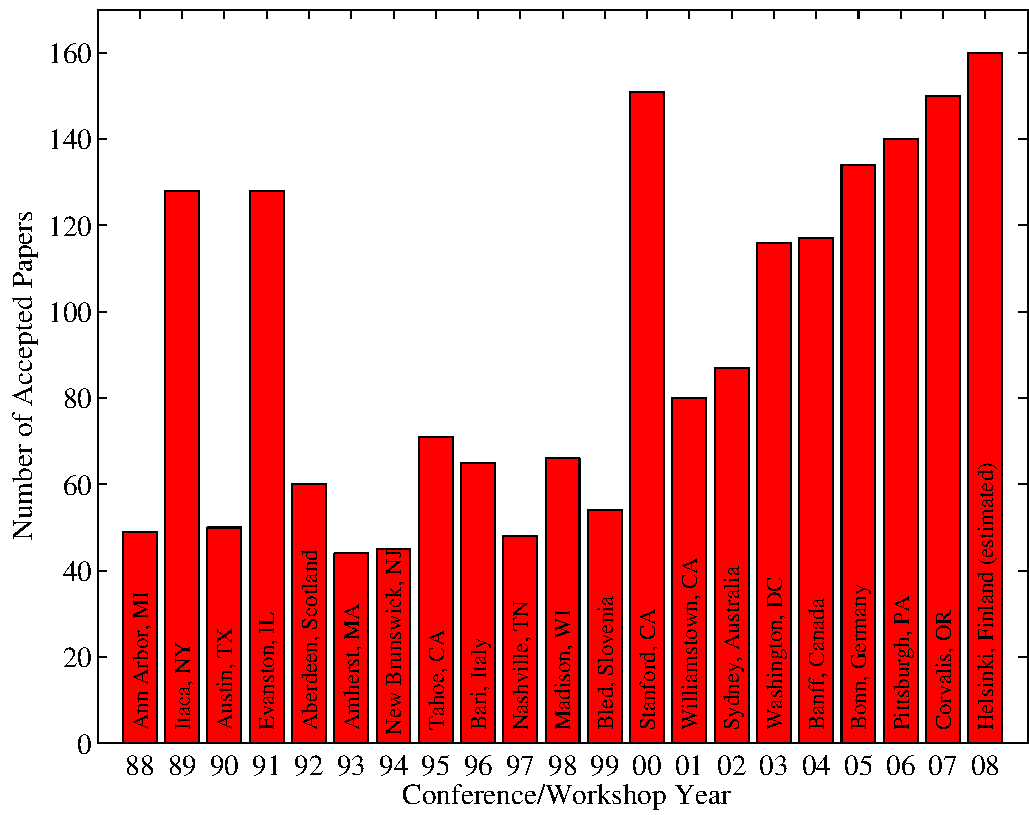
\includegraphics[width=\columnwidth]{icml_numpapers}}
\caption{Historical locations and number of accepted papers for International
Machine Learning Conferences (ICML 1993 -- ICML 2008) and International
Workshops on Machine Learning (ML 1988 -- ML 1992). At the time this figure was
produced, the number of accepted papers for ICML 2008 was unknown and instead
estimated.}
\label{icml-historical}
\end{center}
\vskip -0.2in
\end{figure}

\subsection{Figures}

You may want to include figures in the paper to illustrate
your approach and results. Such artwork should be centered,
legible, and separated from the text. Lines should be dark and at
least 0.5~points thick for purposes of reproduction, and text should
not appear on a gray background.

Label all distinct components of each figure. If the figure takes the
form of a graph, then give a name for each axis and include a legend
that briefly describes each curve. Do not include a title inside the
figure; instead, the caption should serve this function.

Number figures sequentially, placing the figure number and caption
\emph{after} the graphics, with at least 0.1~inches of space before
the caption and 0.1~inches after it, as in
\cref{icml-historical}. The figure caption should be set in
9~point type and centered unless it runs two or more lines, in which
case it should be flush left. You may float figures to the top or
bottom of a column, and you may set wide figures across both columns
(use the environment \texttt{figure*} in \LaTeX). Always place
two-column figures at the top or bottom of the page.

\subsection{Algorithms}

If you are using \LaTeX, please use the ``algorithm'' and ``algorithmic''
environments to format pseudocode. These require
the corresponding stylefiles, algorithm.sty and
algorithmic.sty, which are supplied with this package.
\cref{alg:example} shows an example.

\begin{algorithm}[tb]
   \caption{Bubble Sort}
   \label{alg:example}
\begin{algorithmic}
   \STATE {\bfseries Input:} data $x_i$, size $m$
   \REPEAT
   \STATE Initialize $noChange = true$.
   \FOR{$i=1$ {\bfseries to} $m-1$}
   \IF{$x_i > x_{i+1}$}
   \STATE Swap $x_i$ and $x_{i+1}$
   \STATE $noChange = false$
   \ENDIF
   \ENDFOR
   \UNTIL{$noChange$ is $true$}
\end{algorithmic}
\end{algorithm}

\subsection{Tables}

You may also want to include tables that summarize material. Like
figures, these should be centered, legible, and numbered consecutively.
However, place the title \emph{above} the table with at least
0.1~inches of space before the title and the same after it, as in
\cref{sample-table}. The table title should be set in 9~point
type and centered unless it runs two or more lines, in which case it
should be flush left.

% Note use of \abovespace and \belowspace to get reasonable spacing
% above and below tabular lines.

\begin{table}[t]
\caption{Classification accuracies for naive Bayes and flexible
Bayes on various data sets.}
\label{sample-table}
\vskip 0.15in
\begin{center}
\begin{small}
\begin{sc}
\begin{tabular}{lcccr}
\toprule
Data set & Naive & Flexible & Better? \\
\midrule
Breast    & 95.9$\pm$ 0.2& 96.7$\pm$ 0.2& $\surd$ \\
Cleveland & 83.3$\pm$ 0.6& 80.0$\pm$ 0.6& $\times$\\
Glass2    & 61.9$\pm$ 1.4& 83.8$\pm$ 0.7& $\surd$ \\
Credit    & 74.8$\pm$ 0.5& 78.3$\pm$ 0.6&         \\
Horse     & 73.3$\pm$ 0.9& 69.7$\pm$ 1.0& $\times$\\
Meta      & 67.1$\pm$ 0.6& 76.5$\pm$ 0.5& $\surd$ \\
Pima      & 75.1$\pm$ 0.6& 73.9$\pm$ 0.5&         \\
Vehicle   & 44.9$\pm$ 0.6& 61.5$\pm$ 0.4& $\surd$ \\
\bottomrule
\end{tabular}
\end{sc}
\end{small}
\end{center}
\vskip -0.1in
\end{table}

Tables contain textual material, whereas figures contain graphical material.
Specify the contents of each row and column in the table's topmost
row. Again, you may float tables to a column's top or bottom, and set
wide tables across both columns. Place two-column tables at the
top or bottom of the page.

\subsection{Theorems and such}
The preferred way is to number definitions, propositions, lemmas, etc. consecutively, within sections, as shown below.
\begin{definition}
\label{def:inj}
A function $f:X \to Y$ is injective if for any $x,y\in X$ different, $f(x)\ne f(y)$.
\end{definition}
Using \cref{def:inj} we immediate get the following result:
\begin{proposition}
If $f$ is injective mapping a set $X$ to another set $Y$, 
the cardinality of $Y$ is at least as large as that of $X$
\end{proposition}
\begin{proof} 
Left as an exercise to the reader. 
\end{proof}
\cref{lem:usefullemma} stated next will prove to be useful.
\begin{lemma}
\label{lem:usefullemma}
For any $f:X \to Y$ and $g:Y\to Z$ injective functions, $f \circ g$ is injective.
\end{lemma}
\begin{theorem}
\label{thm:bigtheorem}
If $f:X\to Y$ is bijective, the cardinality of $X$ and $Y$ are the same.
\end{theorem}
An easy corollary of \cref{thm:bigtheorem} is the following:
\begin{corollary}
If $f:X\to Y$ is bijective, 
the cardinality of $X$ is at least as large as that of $Y$.
\end{corollary}
\begin{assumption}
The set $X$ is finite.
\label{ass:xfinite}
\end{assumption}
\begin{remark}
According to some, it is only the finite case (cf. \cref{ass:xfinite}) that is interesting.
\end{remark}
%restatable

\subsection{Citations and References}

Please use APA reference format regardless of your formatter
or word processor. If you rely on the \LaTeX\/ bibliographic
facility, use \texttt{natbib.sty} and \texttt{icml2024.bst}
included in the style-file package to obtain this format.

Citations within the text should include the authors' last names and
year. If the authors' names are included in the sentence, place only
the year in parentheses, for example when referencing Arthur Samuel's
pioneering work \yrcite{Samuel59}. Otherwise place the entire
reference in parentheses with the authors and year separated by a
comma \cite{Samuel59}. List multiple references separated by
semicolons \cite{kearns89,Samuel59,mitchell80}. Use the `et~al.'
construct only for citations with three or more authors or after
listing all authors to a publication in an earlier reference \cite{MachineLearningI}.

Authors should cite their own work in the third person
in the initial version of their paper submitted for blind review.
Please refer to \cref{author info} for detailed instructions on how to
cite your own papers.

Use an unnumbered first-level section heading for the references, and use a
hanging indent style, with the first line of the reference flush against the
left margin and subsequent lines indented by 10 points. The references at the
end of this document give examples for journal articles \cite{Samuel59},
conference publications \cite{langley00}, book chapters \cite{Newell81}, books
\cite{DudaHart2nd}, edited volumes \cite{MachineLearningI}, technical reports
\cite{mitchell80}, and dissertations \cite{kearns89}.

Alphabetize references by the surnames of the first authors, with
single author entries preceding multiple author entries. Order
references for the same authors by year of publication, with the
earliest first. Make sure that each reference includes all relevant
information (e.g., page numbers).

Please put some effort into making references complete, presentable, and
consistent, e.g. use the actual current name of authors.
If using bibtex, please protect capital letters of names and
abbreviations in titles, for example, use \{B\}ayesian or \{L\}ipschitz
in your .bib file.

\section*{Accessibility}
Authors are kindly asked to make their submissions as accessible as possible for everyone including people with disabilities and sensory or neurological differences.
Tips of how to achieve this and what to pay attention to will be provided on the conference website \url{http://icml.cc/}.

\section*{Software and Data}

If a paper is accepted, we strongly encourage the publication of software and data with the
camera-ready version of the paper whenever appropriate. This can be
done by including a URL in the camera-ready copy. However, \textbf{do not}
include URLs that reveal your institution or identity in your
submission for review. Instead, provide an anonymous URL or upload
the material as ``Supplementary Material'' into the OpenReview reviewing
system. Note that reviewers are not required to look at this material
when writing their review.

% Acknowledgements should only appear in the accepted version.
\section*{Acknowledgements}

\textbf{Do not} include acknowledgements in the initial version of
the paper submitted for blind review.

If a paper is accepted, the final camera-ready version can (and
probably should) include acknowledgements. In this case, please
place such acknowledgements in an unnumbered section at the
end of the paper. Typically, this will include thanks to reviewers
who gave useful comments, to colleagues who contributed to the ideas,
and to funding agencies and corporate sponsors that provided financial
support.


% In the unusual situation where you want a paper to appear in the
% references without citing it in the main text, use \nocite
\nocite{langley00}

\bibliography{example_paper}
\bibliographystyle{icml2024}


%%%%%%%%%%%%%%%%%%%%%%%%%%%%%%%%%%%%%%%%%%%%%%%%%%%%%%%%%%%%%%%%%%%%%%%%%%%%%%%
%%%%%%%%%%%%%%%%%%%%%%%%%%%%%%%%%%%%%%%%%%%%%%%%%%%%%%%%%%%%%%%%%%%%%%%%%%%%%%%
% APPENDIX
%%%%%%%%%%%%%%%%%%%%%%%%%%%%%%%%%%%%%%%%%%%%%%%%%%%%%%%%%%%%%%%%%%%%%%%%%%%%%%%
%%%%%%%%%%%%%%%%%%%%%%%%%%%%%%%%%%%%%%%%%%%%%%%%%%%%%%%%%%%%%%%%%%%%%%%%%%%%%%%
\newpage
\appendix
\onecolumn
\section{You \emph{can} have an appendix here.}

You can have as much text here as you want. The main body must be at most $8$ pages long.
For the final version, one more page can be added.
If you want, you can use an appendix like this one.  

The $\mathtt{\backslash onecolumn}$ command above can be kept in place if you prefer a one-column appendix, or can be removed if you prefer a two-column appendix.  Apart from this possible change, the style (font size, spacing, margins, page numbering, etc.) should be kept the same as the main body.
%%%%%%%%%%%%%%%%%%%%%%%%%%%%%%%%%%%%%%%%%%%%%%%%%%%%%%%%%%%%%%%%%%%%%%%%%%%%%%%
%%%%%%%%%%%%%%%%%%%%%%%%%%%%%%%%%%%%%%%%%%%%%%%%%%%%%%%%%%%%%%%%%%%%%%%%%%%%%%%


\end{document}


% This document was modified from the file originally made available by
% Pat Langley and Andrea Danyluk for ICML-2K. This version was created
% by Iain Murray in 2018, and modified by Alexandre Bouchard in
% 2019 and 2021 and by Csaba Szepesvari, Gang Niu and Sivan Sabato in 2022.
% Modified again in 2023 and 2024 by Sivan Sabato and Jonathan Scarlett.
% Previous contributors include Dan Roy, Lise Getoor and Tobias
% Scheffer, which was slightly modified from the 2010 version by
% Thorsten Joachims & Johannes Fuernkranz, slightly modified from the
% 2009 version by Kiri Wagstaff and Sam Roweis's 2008 version, which is
% slightly modified from Prasad Tadepalli's 2007 version which is a
% lightly changed version of the previous year's version by Andrew
% Moore, which was in turn edited from those of Kristian Kersting and
% Codrina Lauth. Alex Smola contributed to the algorithmic style files.
